\documentclass[11pt]{article}

\usepackage{weekly}

\title{Weekly}
\author{Anne Dranowski and Dinushi Munasinghe}
\date{October 2020}

\begin{document}

\maketitle

In these notes we embark on a journey across two major continents: Soergel bimodules and Iwahori--Hecke algebras.

\section*{Goals}

\begin{itemize}
    \item work out at least three constructions of bases in the baby $sl_2$ case 
    \item do the exercises in the SBim textbook
\end{itemize}

% % !TeX root = ./main.tex

Chapter 1 exercises

\begin{enumerate}
    \item[Exercise 1.5] Confirm that the set of all reflections agrees with the set of transpositions $(i,j)$. For each transposition $(i,j)$ with $i<j$, find an expression for it of lenght $2(j-i) - 1$.
    
    \begin{proof}
    First, map simple reflections to simple transpositions $s_i \mapsto (i,i+1)$. 
    Next, extend this map to a homomorphism $\phi$ of $W$ and $S_n$. To check that it extends, let $w\in W$ be an element which is conjugate to a simple reflection, i.e.\ $s_{i_1}\cdots s_{i_a} = w = u s_i u^{-1}$ for some $u = s_{j_1}\cdots s_{j_b}\in W$. Probably it suffices to check the case that $W$ is a product of two simple reflections, so let's start there. If $w = s_p s_q = u\cdot s_i$, then $(p,p+1)(q,q+1)=\phi(u)\cdot (i,i+1)$. 
    \end{proof}
\end{enumerate}

\section*{Day 1}

% 2020-12-28 18:14:34
Reading Mathas: ``very little detailed information is known about the modular representations of the symmetric groups.'' The modular representation theory of the Iwahori--Hecke algebras of the symmetric groups (pioneered by Dipper--James) includes that of $S_n$ as a special ($q=1$) case. ``The main motivation for studying the Iwahori--Hecke algebras is that they provide a bridge between the representation theory of the symmetric and general linear groups''. Schur had classified ordinary irreducible polynomial representations of $\GL_n\CC$ using Schur algebras, so Dipper and James introduced $q$-Schur algebras to study modular rep th of $\GL_n(q)$ over fields of characteristic not dividing $q$ (i.e.\ non-defining characteristic). 

The symmetric group as an abstract group: 
\begin{equation}
    S_n = \left\langle s_1,\dots, s_{n-1} : \begin{aligned}
        s_i^2 &= 1 & i &= 1,\dots, n-1 \\
        s_i s_j &= s_j s_i & |i - j| & \ge 2 \\
        s_i s_{i+1} s_i &= s_{i + 1} s_i s_{i + 1} & i & = 1,2,\dots, n-2 
    \end{aligned}\right\rangle 
\end{equation}
The defining relations can be encoded by the diagrams

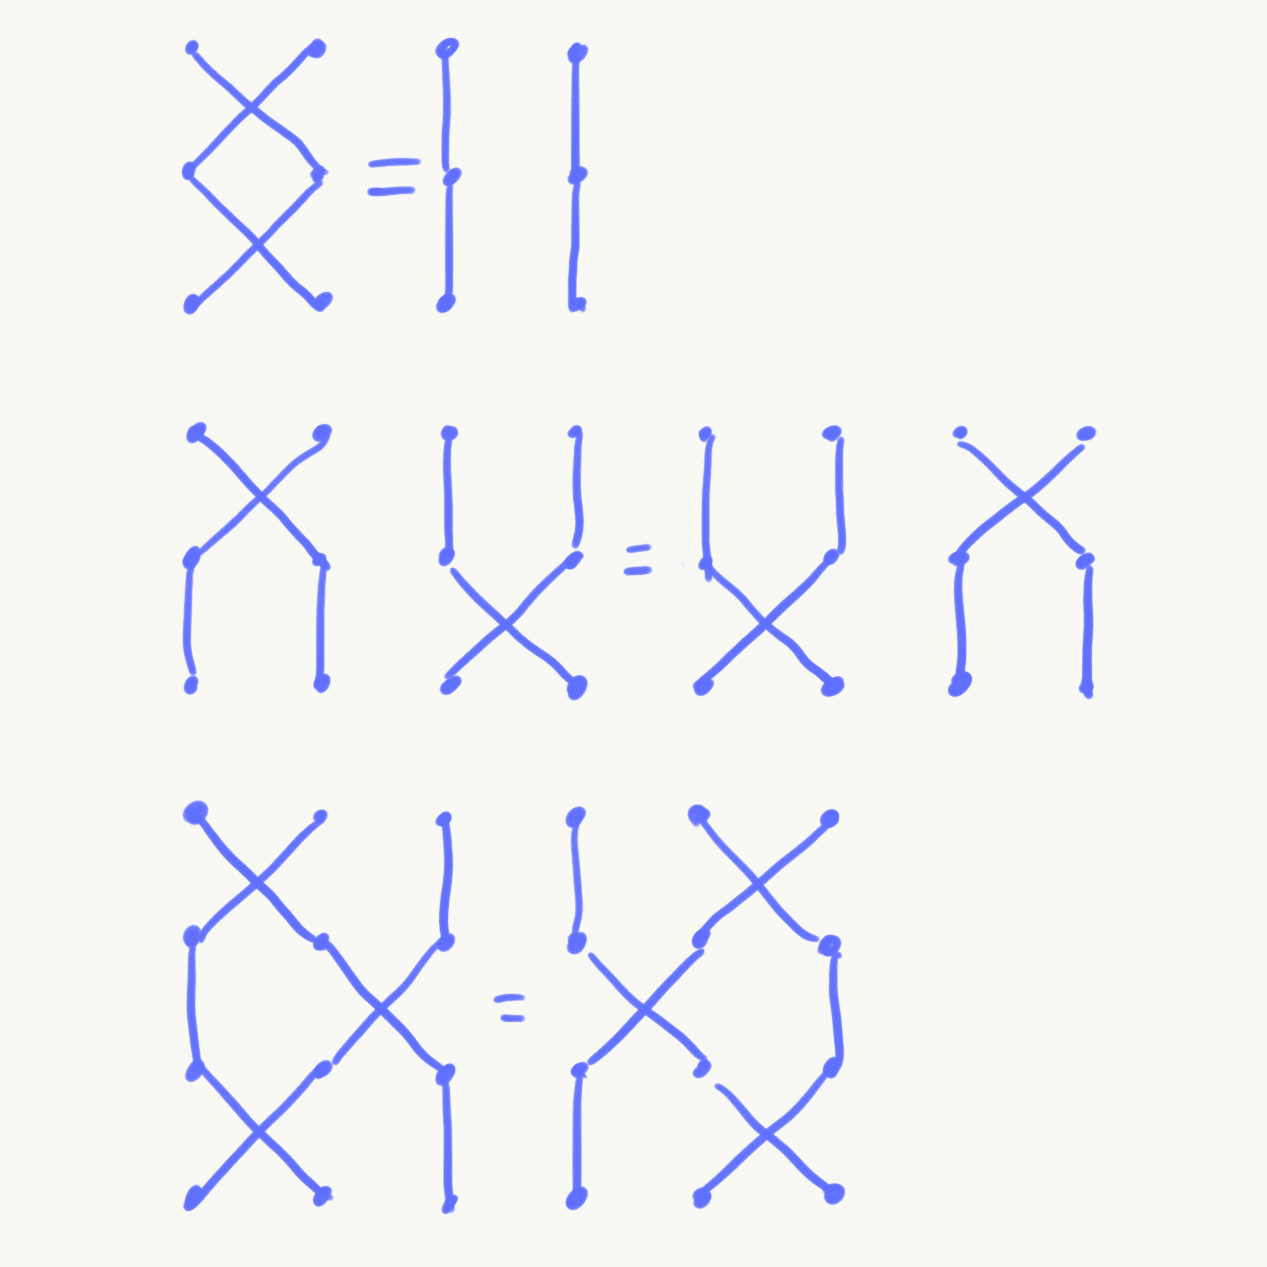
\includegraphics[height=300px]{theSymmetricGroup.png}

One can deform the first relation as follows.
\begin{equation}
    \label{eq:IHrel}
    (T_i - q)(T_i + 1) = 0 
\end{equation}
Note that if we set $q = 1$ we recover $T_i^2 = 1$. On the other hand, if we set $q = 0$ we obtain $T_i^2 = - T_i$ which doesn't look like anything... but apparently arises naturally in the study of the principal series representations of $\GL_n(\FF_q)$. 

\begin{exer}
    Let $\varepsilon : S_n \to \{\pm 1 \}$ denote the sign representation. Recall $\varepsilon$ is defined by setting $\varepsilon(s) = -1$ for all $s\in S = \{s_1,\dots,s_{n-1}\}$. Given $w\in S_n$ show that $\varepsilon(w) = (-1)^{\ell(w)}$ where $\ell$ is the length function. 
\end{exer}

By definition, if $s\in S$ and $w\in S_n$ then $\ell(sw) = \ell(ws) = \ell(w) \pm 1$. 

\begin{exer}
    Prove or disprove the claim that $\ell(sw) = \ell(ws)$ for all $s$, $w$ as above. 
\end{exer}

Let $R$ be a commutative domain with $1$ and let $q\in R$ be arbitrary. The Iwahori--Hecke algebra $\scH = \scH_{R,q}(S_n)$ is the unital associative $R$-algebra having a presentation just like $S_n$ except for the first relation which is replaced by Equation~\ref{eq:IHrel}. I guess for distinction one also uses $T$'s instead of $s$'s to denote the generators of $\scH$. Let's try to rediscover it by recalling Schur--Weyl duality. 

I think that the basic insight in the story of Schur--Weyl duality is this: polynomial rings are symmetric algebras. 

% Let $T\le\GL_n(k)$ be a maximal torus.
Recall that the action of $\GL_n(k)$ on its basic representation $V = k^n$
% $=\spec(k[x_1,\dots,x_n])$ 
dualizes to an action on the polynomial ring $A = k[x_1,\dots,x_n]$
% = k[k^n] 
and $A\cong\sym(V^\ast)$. The dual action is defined with respect to the natural pairing on $\sym(V)\times\sym(V^\ast)$ extending that on $V\times V^\ast$. If we identify $\sym(V)$ with the algebra of constant-coefficient differential operators on $V$, then this pairing is given by 
\begin{equation}
    \sym(V)\times A \to k : (D,f) \mapsto D(f)(0)
\end{equation}
% $A\cong\sym(\lie(T)^\ast)$. 

\begin{exer}
    Actually, the action of $\GL(V)$ extends uniquely to $\sym(V)$ and $A$ by graded algebra automorphisms. The pairing is preserved by this action. 
\end{exer}

\section*{The case $n=2$}

Let $V = k^2$ with its action of $\GL(V) = \GL_2(k)$ and consider $V\otimes V$ as a representation 
\begin{equation}
    g(v_1\otimes v_2) = gv_1\otimes gv_2 
\end{equation}
There is a copy of $S_2$ in $\GL(V)$ and it permutes the tensor factors. So in particular an irreducible subrepresentation of $V$ has to be invariant under this action. So the silliest way to ensure this is to fix a vector (really a tensor product of vectors) and generate as many linearly independent vectors from it by applying the permutation matrices. 

In this case, there's not too many starting points. The basis of the entire tensor product is just 4 vectors. 
\[
\{e_1 \otimes e_1, e_1\otimes e_2, e_2\otimes e_1, e_2\otimes e_2 \}    
\]
From $e_1\otimes e_1$ we can go to $e_2\otimes e_2$ and that's it. So that's one invariant subspace. Similarly from $e_1\otimes e_2$ we can go to $e_2\otimes e_1$ and that's it because there's nothing left. 

\begin{exer}
    If $W\subset V\otimes V$ is invariant under $S_2\le \GL_2$ then it's invariant under $\GL_2$. 
\end{exer}

\begin{exer}
    WTH changes when we work with $\GL_2(q)$?? 
\end{exer}

\section*{On Iwahori--Hecke}



\end{document}
